De manera análoga al caso de espacio libre, se procede a diseñar los adaptadores de cuarto de onda y \texttt{stub}, considerando el valor de carga \ref{ec.z_80_tierra}.

\subsection{Adaptador de cuarto de onda}

%%%% FIGURA PARA STUB CON TIERRA
%\begin{figure}[H]
%	\centering
%	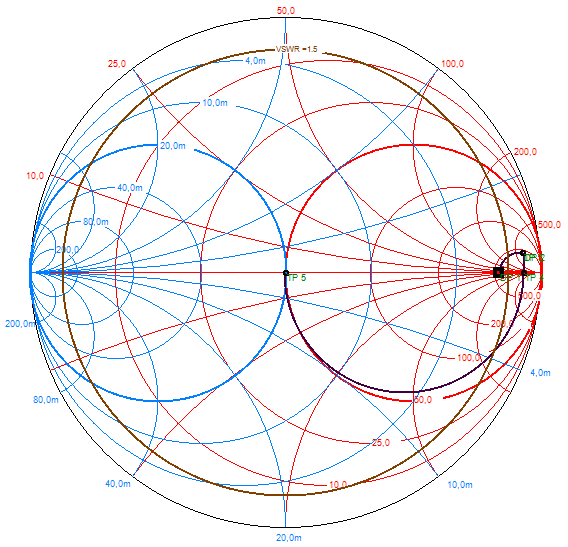
\includegraphics[scale=0.43]{imagenes/smith_4_tierra.png}
%	\label{fig.smith_4_tierra}
%\end{figure}


\subsection{Stub}

%%%% FIGURA PARA STUB CON TIERRA
%\begin{figure}[H]
%	\centering
%	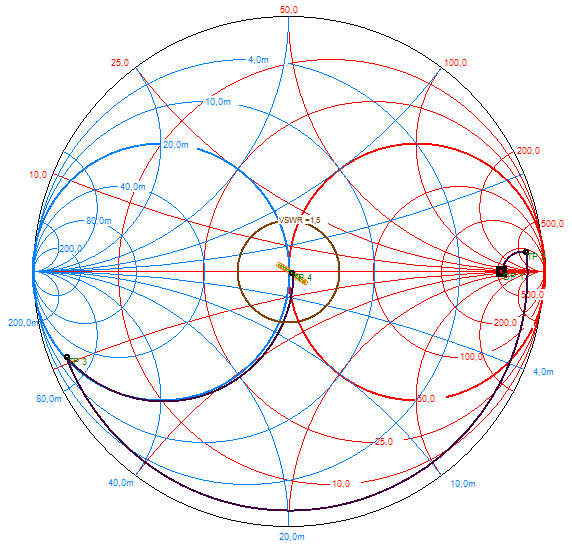
\includegraphics[scale=0.43]{imagenes/smith_stub_tierra.png}
%	\label{fig.smith_stub_tierra}
%\end{figure}